\documentclass{article}

\usepackage{graphicx}
\usepackage{xcolor}
\usepackage{indentfirst}
\usepackage[a4paper, total={6in, 8in}]{geometry}
\usepackage{hyperref}
\usepackage{fancyhdr}
\usepackage{xepersian}
\settextfont{B Nazanin}
\setlatintextfont{Times New Roman}
\renewcommand{\labelitemi}{$\bullet$}

\definecolor{codegray}{gray}{0.9}
\newcommand{\code}[1]{\colorbox{codegray}{\texttt{#1}}}

\begin{document}


%title page%
\begin{titlepage}
	\begin{center}
		\vspace{0.2cm}
		
		
\includegraphics[width=0.4\textwidth]{sharif.png}\\
		\vspace{0.2cm}
		\textbf{ \Huge{آزمایش شماره 4}}\\
		\vspace{0.25cm}
		\textbf{ \Large{آز شبکه - دکتر بردیا صفایی}}
		\vspace{0.2cm}
		
		
		\large \textbf{دانشکده مهندسی کامپیوتر}\\\vspace{0.1cm}
		\large   دانشگاه صنعتی شریف\\\vspace{0.2cm}
		\large   ﻧﯿﻢ‌سال اول ۰۱-۰۲ \\\vspace{0.10cm}
		\large{ گروه 8:}\\
		\large{\href{mailto:mehrshad.mirmohammadi@gmail.com}{مهرشاد میرمحمدی - 98109634}}\\
		\large{\href{mailto:parhaamsaremi@gmail.com}{پرهام صارمی - 97101959}}\\
		\large{\href{mailto:mofayezi.m@gmail.com}{محمدرضا مفیضی - 98106059}}\\
	\end{center}
\end{titlepage}
%title page%

\newpage

%pages header
\pagestyle{fancy}
\fancyhf{}
\fancyfoot{}
\setlength{\headheight}{59pt}
\cfoot{\thepage}
\lhead{آزمایش شماره 4}
\rhead{
\includegraphics[width=0.1\textwidth]{sharif.png}\\
		دانشکده مهندسی کامپیوتر
}
\chead{آز شبکه - گروه 8}
%pages header

\section{پیاده‌سازی}
ابتدا در محیط \lr{packet tracer} سناریو اول گفته شده در کلاس را طراحی می‌کنیم.
\begin{figure}[h!]
	\centering
	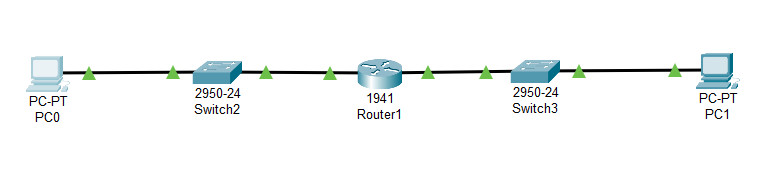
\includegraphics[width=0.6\columnwidth]{figs/scenario-1.jpg}
	\caption{تصویر پیاده‌سازی سناریو اول در محیط \lr{packet tracer}}
	\label{fig:scenario-1}
\end{figure}

برای این‌کار ابتدا در بخش \lr{IP Configuration} آدرس \lr{PC}ها را با مقادیر \code{\lr{192.168.1.2}} و \code{\lr{192.168.2.2}} تنظیم ‌می‌کنیم. (\lr{Subnet Mask} و \lr{Default Gateway} را هم مطابق توضیحات کلاس تنظیم می‌کنیم)

سپس در روتر \lr{interface}ها را مطابق شکل \ref{fig:router-config} تعریف می‌کنیم و با دستور \code{\lr{no shutdown}} آن‌ها را روشن می‌کنیم.
\begin{figure}[h!]
	\centering
	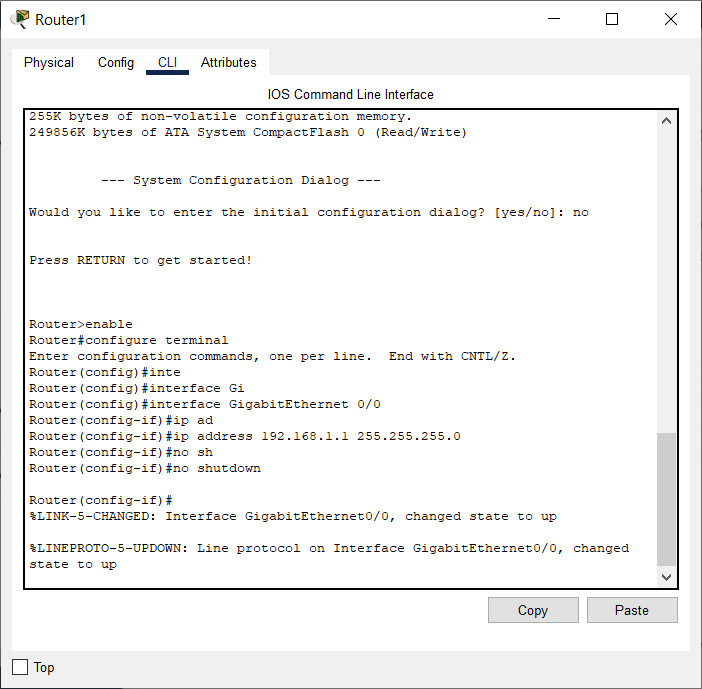
\includegraphics[width=0.6\columnwidth]{figs/router-config.jpg}
	\caption{روشن‌کردن \lr{interface}های روتر}
	\label{fig:router-config}
\end{figure}

حالا می‌توانیم مطابق شکل \ref{fig:ping-1} از \lr{PC1} دستگاه \lr{PC2} را \lr{ping} کنیم.
\begin{figure}[h!]
	\centering
	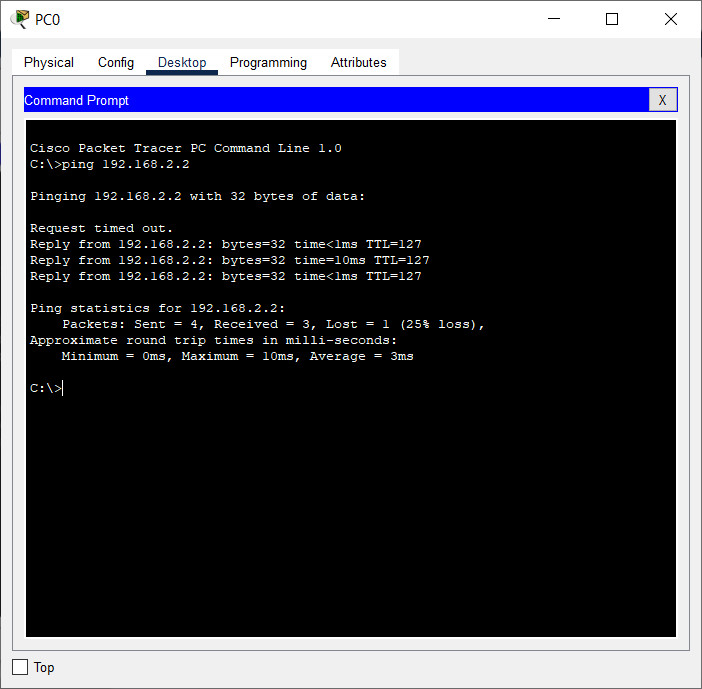
\includegraphics[width=0.6\columnwidth]{figs/ping-1.jpg}
	\caption{\lr{ping} کردن \lr{192.168.2.2}}
	\label{fig:ping-1}
\end{figure}

در سناریو بعدی (شکل \ref{fig:scenario-2}) باید دو روتر را با کابل سریال به هم متصل کنیم. از آن‌جایی که روتر \lr{2621XM} پورت سریال ندارد، ابتدا ماژول \lr{WIC-2T} را به آن اضافه می‌کنیم.
\begin{figure}[h!]
	\centering
	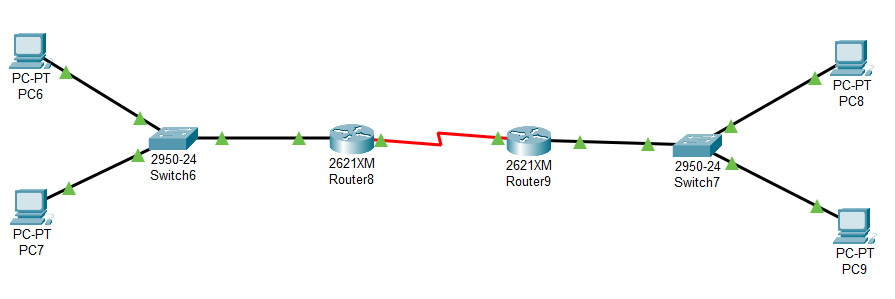
\includegraphics[width=0.6\columnwidth]{figs/scenario-2.jpg}
	\caption{پیاده‌سازی سناریو دوم}
	\label{fig:scenario-2}
\end{figure}

سپس روترها را از طریق \lr{interface}های سریال به هم وصل و پیکربندی می‌کنیم. 
حالا مطابق شکل \ref{fig:serial-route} با روش روتینگ استاتیک شبکه‌ها را به هم می‌شناسانیم.

\begin{figure}[h!]
	\centering
	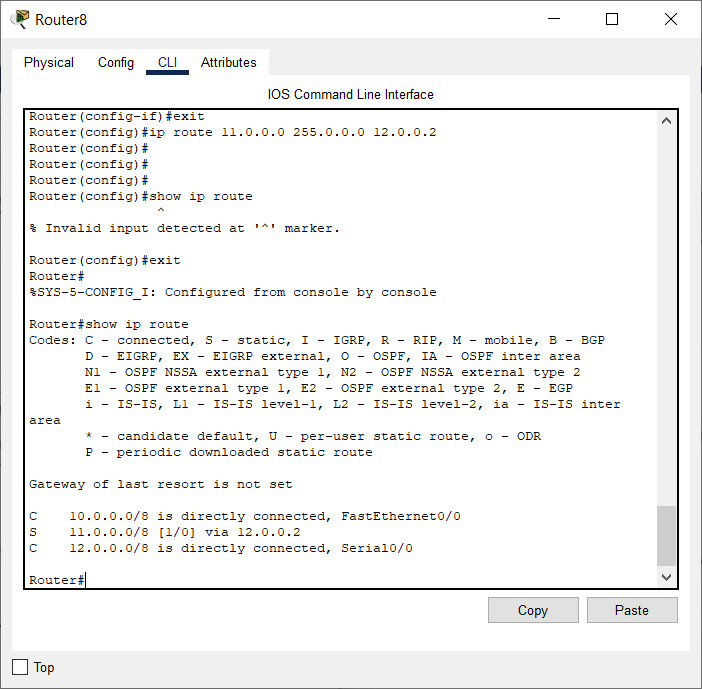
\includegraphics[width=0.6\columnwidth]{figs/serial-route.jpg}
	\caption{نمایش روتینگ استاتیک اضافه‌شده با دستور \code{\lr{show ip route}}}
	\label{fig:serial-route}
\end{figure}


\section{محیط \lr{CLI} سوئیچ}

مطابق شکل \ref{fig:user-excec-commands} در منوی \lr{CLI} با زدن دستور \code{?} لیست دستورات قابل اجرا در محیط \lr{User EXEC} را مشاهده می‌کنیم.
\begin{figure}[h!]
	\centering
	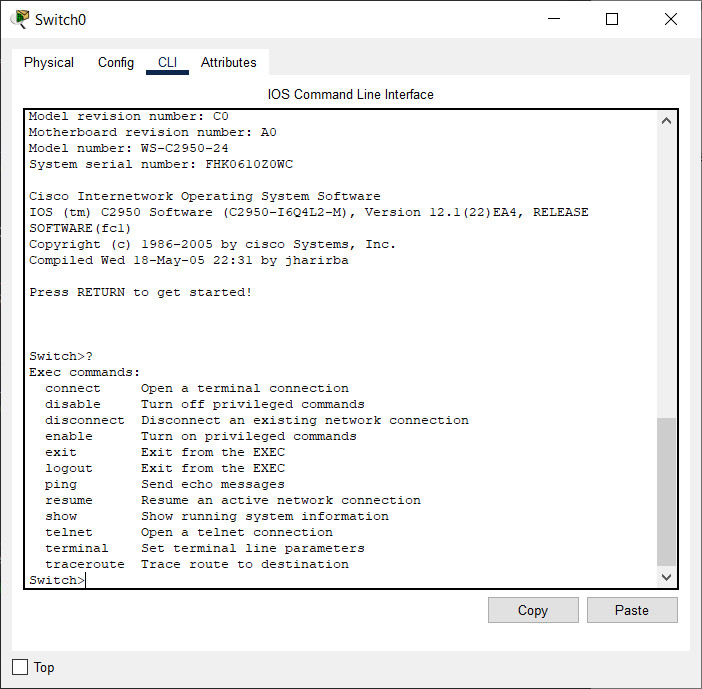
\includegraphics[width=0.6\columnwidth]{figs/user-excec-commands.jpg}
	\caption{لیست دستورات قابل اجرا در محیط \lr{User EXEC}}
	\label{fig:user-excec-commands}
\end{figure}

هر کدام از دستورات شکل بالا به صورت زیر عمل می‌کند:
\begin{itemize}
	\item 
	دستور \code{connect} اتصالی جدید به یک \lr{terminal} ایجاد می‌کند.
	\item 
	دستور \code{disable} برای خروج از حالت \lr{privileged} و غیرفعال کردن دستورات آن به‌کار برده می‌شود.
	\item 
	دستور \code{disconnect} درست برعکس دستور \code{connect} اتصال فعلی را قطع می‌کند.
	\item 
	دستور \code{enable} نیز برعکس دستور \code{disable} برای ورود به حالت \lr{privileged} و فعال کردن دستورات آن استفاده می‌شود.
	\item 
	دستورات \code{exit}  و \code{logout} برای خروج از حالت \lr{User EXCEC} و بستن \lr{CLI} استفاده می‌شود.
	\item 
	دستور \code{ping} برای ارسال بسته‌های \lr{echo} به شبکه برای بررسی اتصال شبکه و تاخیر در آن استفاده می‌شود.
	\item 
	دستور \code{resume} برای از سر گیری اتصال فعال شبکه استفاده می‌شود.
	\item 
	دستور \code{show} برای نمایش اطلاعات سیستم درحال اجرا استفاده می‌شود.
	\item 
	دستور \code{telnet} برای ایجاد یک ارتباط \lr{telnet} و برقراری ارتباط با یک دستگاه دیگر استفاده می‌شود.
	\item 
	دستور \code{terminal} برای تعیین پارامترهای خطوط ترمینال است.
	\item 
	دستور \code{traceroute} برای بررسی مسیر یک بسته در شبکه و محاسبه تاخیر آن تا یک دستگاه دیگر استفاده می‌شود.
\end{itemize}

با دستور \code{enable} وارد محیط \lr{Previlaged EXEC} می‌شویم. 
سپس دستورات \code{show} را اجرا می‌کنیم:
\begin{itemize}
	\item 
	\code{\lr{show running-config}}
	تصویر \ref{fig:show-running-config}.
	\begin{figure}[h!]
		\centering
		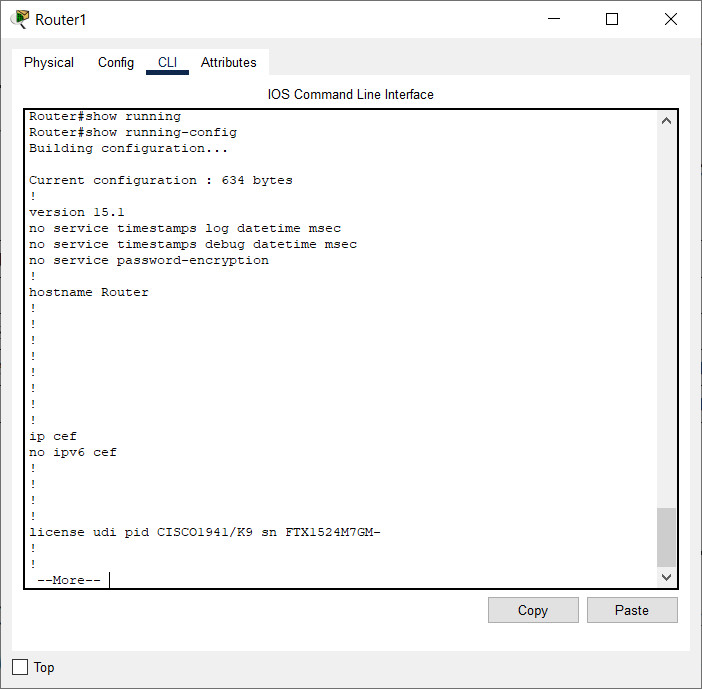
\includegraphics[width=0.6\columnwidth]{figs/show-running-config.jpg}
		\caption{اجرای دستور \code{\lr{show running-config}}}
		\label{fig:show-running-config}
	\end{figure}
	\item 
	\code{\lr{show ip route}}
	تصویر \ref{fig:show-ip-route}.
	\begin{figure}[h!]
		\centering
		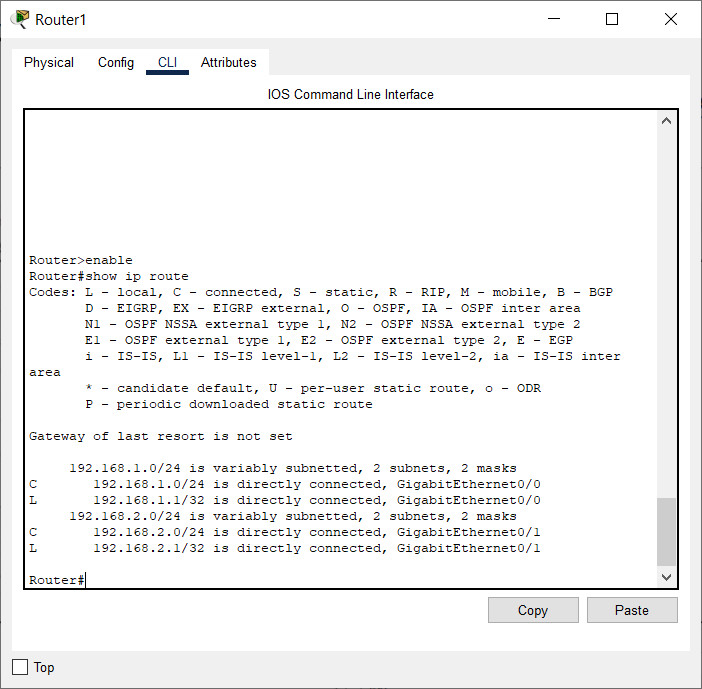
\includegraphics[width=0.6\columnwidth]{figs/show-ip-route.jpg}
		\caption{اجرای دستور \code{\lr{show ip route}}}
		\label{fig:show-ip-route}
	\end{figure}
	\item 
	\code{\lr{show mac address-table}}
	تصویر \ref{fig:show-mac-table}.
	\begin{figure}[h!]
		\centering
		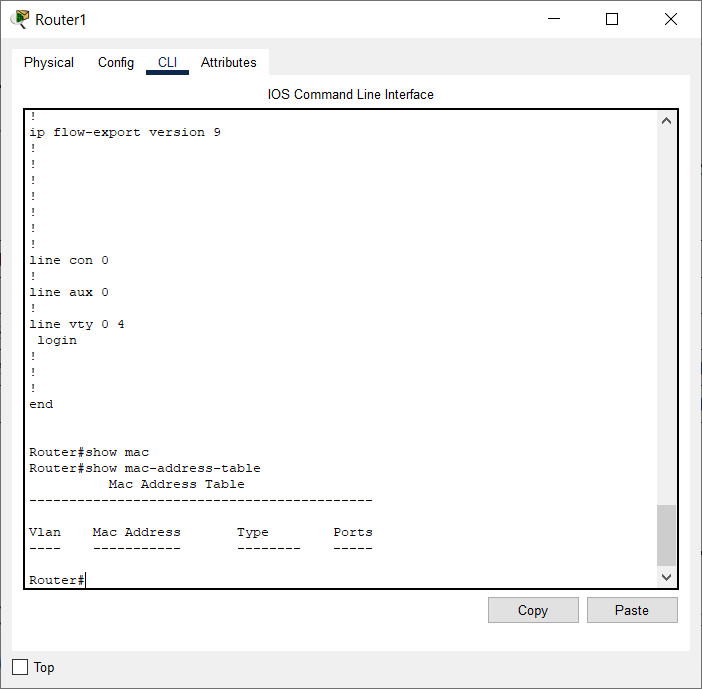
\includegraphics[width=0.6\columnwidth]{figs/show-mac-table.jpg}
		\caption{اجرای دستور \code{\lr{show mac address-table}}}
		\label{fig:show-mac-table}
	\end{figure}
	\item 
	\code{\lr{show ip interface brief}}
	تصویر \ref{fig:show-ip-interface}.
	\begin{figure}[h!]
		\centering
		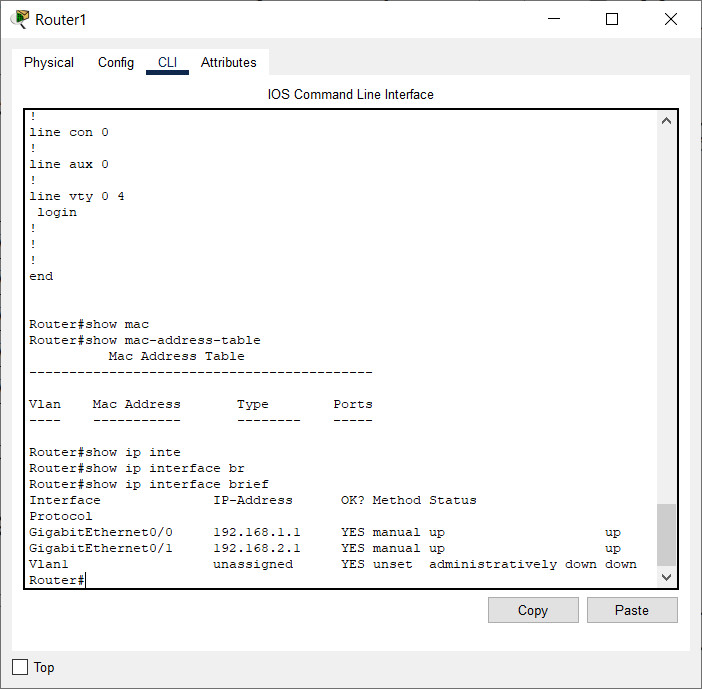
\includegraphics[width=0.6\columnwidth]{figs/show-ip-interface.jpg}
		\caption{اجرای دستور \code{\lr{show ip interface brief}}}
		\label{fig:show-ip-interface}
	\end{figure}
	\item 
	\code{\lr{show vlan brief}}
	تصویر \ref{fig:show-vlan-brief}.
	\begin{figure}[h!]
		\centering
		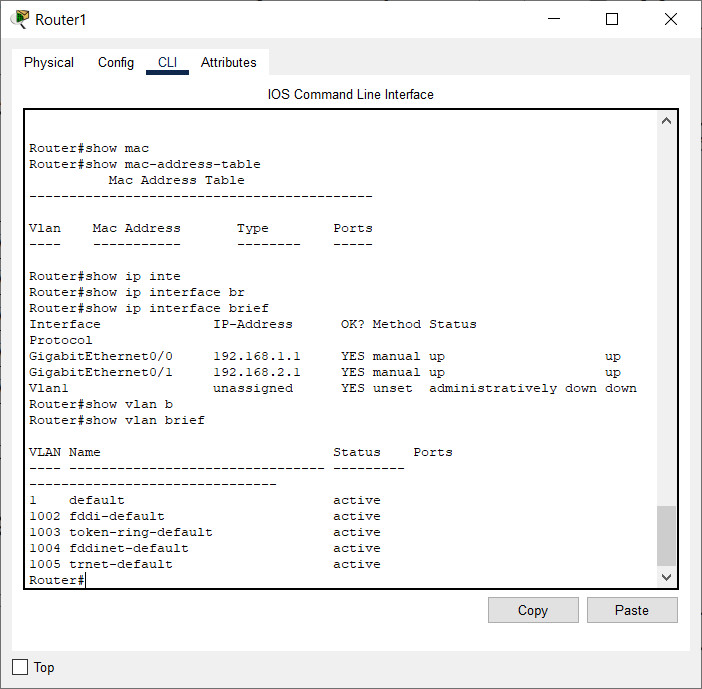
\includegraphics[width=0.6\columnwidth]{figs/show-vlan-brief.jpg}
		\caption{اجرای دستور \code{\lr{show vlan brief}}}
		\label{fig:show-vlan-brief}
	\end{figure}
\end{itemize}

\section{\lr{Gateway} چیست؟}
\lr{Gateway}
 بخشی از یک شبکه است که گذرگاهی بین دو شبکه با پروتکل‌های انتقال مختلف ایجاد می‌کند. بسته به نوع عملکرد، یک \lr{Gateway} می‌تواند در هر یک از هفت لایه مدل \lr{OSI} کار کند. \lr{Gateway} به عنوان نقطه ورود یا خروج یک شبکه عمل می‌کند زیرا تمام ترافیکی که در شبکه‌ها جریان دارد باید از \lr{Gateway} عبور کند. فقط ترافیک داخلی بین نودهای یک \lr{LAN} از \lr{Gateway} عبور نمی‌کند. 
 
 
 

\end{document}
